\documentclass[11pt,a4paper]{article}

\usepackage[T1]{fontenc}
\usepackage[utf8]{inputenc}
\usepackage[main=italian,provide=*]{babel}
\usepackage{amsmath,amssymb}
\usepackage[a4paper,margin=2.3cm]{geometry}
\usepackage{siunitx}
\usepackage{enumitem}
\usepackage{tikz}
\usepackage{xcolor}
\usepackage{fancyhdr}
\usepackage{titlesec}

\sisetup{output-decimal-marker={,},per-mode=symbol,separate-uncertainty=true}
\usetikzlibrary{angles,quotes}

% ---- stile ----
\definecolor{blu}{RGB}{20,60,120}
\titleformat{\section}{\normalfont\large\bfseries\color{blu}}{\thesection.}{0.6em}{}
\titleformat{\subsection}{\normalfont\bfseries}{}{0em}{}
\setlist[enumerate]{leftmargin=1.7em,itemsep=3pt,topsep=3pt}

\pagestyle{fancy}
\fancyhf{}
\lhead{\small Liceo Scientifico ``G.\ Galilei''}
\rhead{\small Fisica -- ripasso estivo}
\cfoot{\small\thepage}
\renewcommand{\headrulewidth}{0.4pt}

\newcommand{\risultato}[1]{\par\smallskip\hfill\emph{[Risultato: #1]}}
\newcommand{\es}{\refstepcounter{esnum}\medskip\noindent\textbf{Esercizio~\theesnum.}\ }
\newcounter{esnum}[section]
\renewcommand{\theesnum}{\thesection.\arabic{esnum}}

\begin{document}

% ================= INTESTAZIONE =================
\begin{center}
  {\LARGE\bfseries\color{blu} Scheda di ripasso di Fisica}\\[2pt]
  {\large In preparazione alla classe terza  A.S.\ 2025/26}\\[6pt]
    
\end{center}

\noindent\rule{\textwidth}{0.8pt}

\medskip
\noindent


% ================= 1. VETTORI =================
\section{Vettori e scomposizione}

\es Una velocità di modulo $v = \SI{20}{\meter\per\second}$ è inclinata di $\ang{35}$ rispetto
all'orizzontale. Determina le sue componenti orizzontale ($v_x$) e verticale ($v_y$).

\es Un blocco è appoggiato su un piano inclinato di $\ang{20}$. Sul blocco agisce il peso
$P = \SI{25}{\newton}$, diretto verticalmente verso il basso. Scomponi il peso lungo la direzione
\emph{parallela} al piano e lungo quella \emph{perpendicolare} al piano.

\es Su un punto materiale agiscono due forze complanari: $F_1 = \SI{12}{\newton}$ diretta lungo
l'asse $x$ e $F_2 = \SI{9}{\newton}$ che forma un angolo di $\ang{60}$ con $F_1$. Determina il
modulo della forza risultante e l'angolo che essa forma con l'asse $x$.

\begin{center}
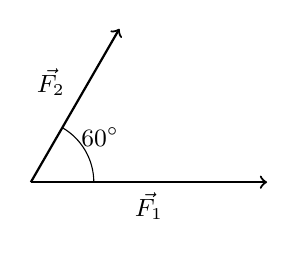
\begin{tikzpicture}[scale=1]
  \draw[->,thick] (0,0)--(3,0) node[midway,below]{\small $\vec{F_1}$};
  \draw[->,thick] (0,0)--(60:2.25) node[midway,above left]{\small $\vec{F_2}$};
  \draw (0.8,0) arc (0:60:0.8);
  \node at (33:1.05) {\small $\ang{60}$};
\end{tikzpicture}
\end{center}

% ================= 2. CINEMATICA RETTILINEA =================
\section{Cinematica rettilinea}

\es Un'automobile parte da ferma e accelera uniformemente con $a = \SI{2,5}{\meter\per\second\squared}$.
Calcola la velocità raggiunta e lo spazio percorso dopo $t = \SI{6,0}{\second}$.

\es Due automobili viaggiano nello stesso verso lungo una strada rettilinea, con velocità costanti.
L'auto A viaggia a $\SI{20}{\meter\per\second}$; nell'istante iniziale si trova $\SI{120}{\meter}$
dietro l'auto B, che procede a $\SI{12}{\meter\per\second}$. Fissata l'origine sulla posizione
iniziale di A:
\begin{enumerate}[label=\alph*)]
  \item scrivi le leggi orarie delle due automobili;
  \item determina dopo quanto tempo A raggiunge B e in quale posizione avviene il sorpasso.
\end{enumerate}

\es Una pallina viene lanciata verticalmente verso l'alto con velocità iniziale
$v_0 = \SI{12}{\meter\per\second}$. Trascurando l'attrito dell'aria, calcola l'altezza massima
raggiunta, il tempo di salita e il tempo totale di volo (fino al ritorno al punto di lancio).

% ================= 3. MOTO CIRCOLARE =================
\section{Cinematica nel piano: moto circolare uniforme}

\es Una ruota di raggio $r = \SI{0,40}{\meter}$ ruota a regime costante compiendo
$\num{300}$ giri al minuto (rpm). Calcola la frequenza, il periodo, la velocità angolare, la
velocità di un punto del bordo e la sua accelerazione centripeta.

\es Un corpo percorre una circonferenza di raggio $r = \SI{2,5}{\meter}$ con velocità di modulo
costante $v = \SI{8,0}{\meter\per\second}$. Determina il periodo, la frequenza, la velocità
angolare e l'accelerazione centripeta.

% ================= 4. DINAMICA =================
\section{Dinamica sul piano inclinato}
\textit{\small (stessa impostazione degli esercizi di terza: schema delle forze, poi legge di Newton)}

\es Un oggetto di massa $m = \SI{2,0}{\kilo\gram}$ viene lanciato \emph{dalla base} di un piano
inclinato ($\alpha = \ang{25}$) con velocità iniziale $v_0 = \SI{4,0}{\meter\per\second}$ diretta
lungo il piano, verso l'alto. Il coefficiente di attrito dinamico tra oggetto e piano vale
$\mu_d = 0{,}30$ e la lunghezza del piano è $L = \SI{0,80}{\meter}$.
\begin{enumerate}[label=\arabic*)]
  \item Disegna tutte le forze applicate all'oggetto durante la salita.
  \item Calcola il modulo della forza di attrito dinamico.
  \item Determina il vettore accelerazione (direzione, verso e modulo).
  \item Verifica che l'oggetto raggiunge la sommità e calcola dopo quanto tempo vi arriva e con
        quale velocità.
\end{enumerate}

\begin{center}
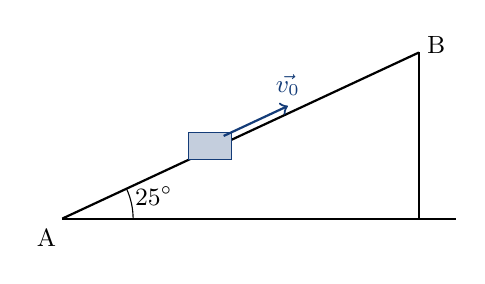
\begin{tikzpicture}[scale=1]
  \draw[thick] (0,0)--(5,0);
  \draw[thick] (0,0)--(4.53,2.11);
  \draw[thick] (4.53,2.11)--(4.53,0);
  \draw (0.9,0) arc (0:25:0.9);
  \node at (14:1.2) {\small $\ang{25}$};
  \fill[blu!25,draw=blu] (1.6,0.746) rectangle ++(0.55,0.35);
  \draw[->,thick,blu] (2.05,1.05) -- ++(25:0.9) node[above]{\small $\vec{v_0}$};
  \node at (-0.2,-0.25){\small A}; \node at (4.75,2.2){\small B};
\end{tikzpicture}
\end{center}

% ================= 5. LAVORO ED ENERGIA =================
\section{Lavoro ed energia}

\es Un blocco di massa $m = \SI{3,0}{\kilo\gram}$, inizialmente fermo, scende lungo un piano
inclinato di $\ang{30}$ e lungo $L = \SI{5,0}{\meter}$. Il coefficiente di attrito dinamico tra
blocco e piano vale $\mu_d = 0{,}25$.
\begin{enumerate}[label=\alph*)]
  \item Disegna le forze applicate al blocco mentre scende.
  \item Calcola separatamente il lavoro compiuto dalla forza-peso, dalla reazione normale e dalla
        forza di attrito dinamico lungo il piano.
  \item Usando il teorema dell'energia cinetica, determina la velocità con cui il blocco arriva
        alla base del piano.
\end{enumerate}

\medskip
\noindent\textbf{Sfida (facoltativa).}\ Alla base del piano il blocco prosegue su un tratto
orizzontale liscio (attrito trascurabile) e va a comprimere una molla di costante elastica
$k = \SI{800}{\newton\per\meter}$. Di quanto viene compressa la molla nel punto di massima
compressione? \emph{(Suggerimento: tutta l'energia cinetica si trasforma in energia elastica.
L'energia elastica la studierai meglio in terza, ma la formula è $E_{el}=\tfrac{1}{2}kx^2$.)}

\vfill
\noindent\rule{\textwidth}{0.4pt}
\begin{center}\small Le soluzioni sono nella pagina seguente: provaci prima da sola!\end{center}

\newpage
% ================= SOLUZIONI =================
\begingroup
\color{blu}\section*{\color{blu}Soluzioni}
\endgroup
\setcounter{section}{0}
\renewcommand{\theesnum}{\thesection.\arabic{esnum}}

\subsection*{1 -- Vettori e scomposizione}
\setcounter{section}{1}\setcounter{esnum}{0}

\es $v_x = v\cos\ang{35} = \SI{20}{}\cdot 0{,}819 \approx \SI{16,4}{\meter\per\second}$; \quad
$v_y = v\sin\ang{35} = \SI{20}{}\cdot 0{,}574 \approx \SI{11,5}{\meter\per\second}$.

\es Componente parallela al piano: $P_\parallel = P\sin\ang{20} = 25\cdot 0{,}342 \approx \SI{8,6}{\newton}$;\\
componente perpendicolare: $P_\perp = P\cos\ang{20} = 25\cdot 0{,}940 \approx \SI{23,5}{\newton}$.\\
\emph{(È la stessa scomposizione che userai per il peso sul piano inclinato in dinamica.)}

\es $R_x = F_1 + F_2\cos\ang{60} = 12 + 9\cdot 0{,}5 = \SI{16,5}{\newton}$;\quad
$R_y = F_2\sin\ang{60} = 9\cdot 0{,}866 = \SI{7,79}{\newton}$.\\
$R = \sqrt{R_x^2+R_y^2} = \sqrt{16{,}5^2+7{,}79^2}\approx \SI{18,2}{\newton}$;\quad
$\theta = \arctan\!\frac{R_y}{R_x} = \arctan 0{,}472 \approx \ang{25,3}$.

\subsection*{2 -- Cinematica rettilinea}
\setcounter{section}{2}\setcounter{esnum}{0}

\es $v = a\,t = 2{,}5\cdot 6{,}0 = \SI{15}{\meter\per\second}$;\quad
$s = \tfrac12 a t^2 = \tfrac12\cdot 2{,}5\cdot 6{,}0^2 = \SI{45}{\meter}$.

\es a) $x_A(t) = 20\,t$;\quad $x_B(t) = 120 + 12\,t$ (in metri e secondi).\\
b) Al sorpasso $x_A = x_B$: $\;20t = 120 + 12t \Rightarrow 8t = 120 \Rightarrow t = \SI{15}{\second}$.\\
Posizione: $x = 20\cdot 15 = \SI{300}{\meter}$ dall'origine.

\es $h_{max} = \dfrac{v_0^2}{2g} = \dfrac{12^2}{2\cdot 9{,}81} \approx \SI{7,3}{\meter}$;\quad
$t_{salita} = \dfrac{v_0}{g} = \dfrac{12}{9{,}81}\approx \SI{1,22}{\second}$;\quad
$t_{volo} = 2\,t_{salita} \approx \SI{2,4}{\second}$.

\subsection*{3 -- Moto circolare uniforme}
\setcounter{section}{3}\setcounter{esnum}{0}

\es $f = \dfrac{300}{60} = \SI{5,0}{\hertz}$;\quad $T = \dfrac1f = \SI{0,20}{\second}$;\quad
$\omega = 2\pi f \approx \SI{31,4}{\radian\per\second}$;\\
$v = \omega r = 31{,}4\cdot 0{,}40 \approx \SI{12,6}{\meter\per\second}$;\quad
$a_c = \omega^2 r \approx \SI{395}{\meter\per\second\squared}$.

\es $T = \dfrac{2\pi r}{v} = \dfrac{2\pi\cdot 2{,}5}{8{,}0}\approx \SI{1,96}{\second}$;\quad
$f = \dfrac1T \approx \SI{0,51}{\hertz}$;\quad
$\omega = \dfrac vr = \dfrac{8{,}0}{2{,}5} = \SI{3,2}{\radian\per\second}$;\quad
$a_c = \dfrac{v^2}{r} = \dfrac{64}{2{,}5} = \SI{25,6}{\meter\per\second\squared}$.

\subsection*{4 -- Dinamica sul piano inclinato}
\setcounter{section}{4}\setcounter{esnum}{0}

\es \textbf{Forze:} peso $\vec P$ (verticale), reazione normale $\vec N$ (perpendicolare al piano),
attrito dinamico $\vec f_d$. In salita il moto è verso l'alto, quindi \emph{sia} la componente del
peso lungo il piano \emph{sia} l'attrito sono diretti verso il basso.

\smallskip
Componenti del peso: $P_\parallel = mg\sin\alpha = 2{,}0\cdot 9{,}81\cdot\sin\ang{25} \approx \SI{8,29}{\newton}$;\quad
$N = mg\cos\alpha \approx \SI{17,8}{\newton}$.

\smallskip
\textbf{2)}\; $f_d = \mu_d N = 0{,}30\cdot 17{,}8 \approx \SI{5,3}{\newton}$.

\smallskip
\textbf{3)}\; La forza risultante lungo il piano (verso il basso) vale
$F = P_\parallel + f_d = 8{,}29 + 5{,}33 = \SI{13,6}{\newton}$; quindi
\[
a = \frac{F}{m} = \frac{13{,}6}{2{,}0} \approx \SI{6,8}{\meter\per\second\squared},
\]
diretta \emph{lungo il piano, verso il basso} (decelera l'oggetto che sale).

\smallskip
\textbf{4)}\; Spazio massimo prima di fermarsi: $d = \dfrac{v_0^2}{2a} = \dfrac{16}{13{,}6}\approx \SI{1,17}{\meter} > L$:
quindi l'oggetto \emph{raggiunge la sommità}.\\
Tempo per percorrere $L = \SI{0,80}{\meter}$: da $L = v_0 t - \tfrac12 a t^2$ si ottiene
$3{,}41\,t^2 - 4{,}0\,t + 0{,}80 = 0 \Rightarrow t \approx \SI{0,26}{\second}$.\\
Velocità in sommità: $v = \sqrt{v_0^2 - 2aL} = \sqrt{16 - 10{,}9} \approx \SI{2,3}{\meter\per\second}$.

\subsection*{5 -- Lavoro ed energia}
\setcounter{section}{5}\setcounter{esnum}{0}

\es \textbf{Forze in discesa:} peso $\vec P$, reazione normale $\vec N$, attrito dinamico $\vec f_d$
(diretto verso l'alto lungo il piano, perché il blocco scende).

\smallskip
\textbf{Lavori lungo il piano} (spostamento $L = \SI{5,0}{\meter}$ verso il basso):
\begin{itemize}[leftmargin=1.5em,itemsep=2pt]
  \item Forza-peso: $W_P = mg\sin\alpha\cdot L = 3{,}0\cdot 9{,}81\cdot\sin\ang{30}\cdot 5{,}0 \approx \SI{+73,6}{\joule}$ (motore).
  \item Reazione normale: $W_N = 0$ (perpendicolare allo spostamento).
  \item Attrito dinamico: $f_d = \mu_d\,mg\cos\alpha = 0{,}25\cdot 3{,}0\cdot 9{,}81\cdot\cos\ang{30} \approx \SI{6,37}{\newton}$;\\
        $W_f = -f_d\,L \approx \SI{-31,9}{\joule}$ (resistente).
\end{itemize}

\textbf{Velocità alla base} (teorema dell'energia cinetica, partenza da fermo):
\[
\tfrac12 m v^2 = W_P + W_N + W_f = 73{,}6 - 31{,}9 = \SI{41,7}{\joule}
\;\Rightarrow\;
v = \sqrt{\frac{2\cdot 41{,}7}{3{,}0}} \approx \SI{5,3}{\meter\per\second}.
\]

\smallskip
\textbf{Sfida.}\ Conservazione dell'energia sul tratto liscio: $\tfrac12 m v^2 = \tfrac12 k x^2$, da cui
\[
x = v\sqrt{\frac{m}{k}} = 5{,}27\sqrt{\frac{3{,}0}{800}} \approx \SI{0,32}{\meter}.
\]

\vfill
\noindent\rule{\textwidth}{0.4pt}
\begin{center}\small
Se un esercizio non ti torna, segna dove ti blocchi: ne parliamo volentieri a settembre.
\end{center}

\end{document}